\documentclass{article}
\usepackage[utf8]{inputenc}

\usepackage{hyperref}
\usepackage{tikz}
\usepackage{fullpage}
\usepackage{amsmath}
\usepackage{subfig}
\usepackage{multicol}
\usepackage[ruled,vlined]{algorithm2e}
\usepackage{biblatex}



\bibliography{refs} % Entries are in the "refs.bib" file


\usetikzlibrary{arrows.meta,positioning}

% Modelling Vaccination Prioritisation through a multi population time-varying SVIRD model
% Vaccination Prioritisation: Young vs Old
\title{SARS-CoV-2: Protection vs Prevention}
\author{James Arthur, Ed Keall and Katie Murray}
\date{March 2021}

\begin{document}

\maketitle\newpage
\tableofcontents\listoffigures
\newpage

\newpage 
\section{Introduction}
It has been almost a year since SARS-CoV-2 was defined as a pandemic, with several vaccines that have passed the regulatory checks and data starting to come in about their use, it seems an appropriate time to reconsider the vaccine strategy that we are following and to see if the data still holds to the system. \\

\noindent
This work follows the aim to investigate who to vaccinate initially in a pandemic to minimise the death rate of the total population, with specific focus on the SARS-CoV-2 virus in the UK. We will discuss whether it is optimal, for minimising deaths, to focus on preventing the spread or protecting vulnerable populations (people of 80+ years). If preventing the spread of the disease is favoured over protecting vulnerable populations, then the best strategy would be to vaccinate the ``super-spreaders'' first. However, if protecting vulnerable populations is better to minimise overall deaths, then the best strategy would be to vaccinate these vulnerable populations first. The term ``super-spreaders'' refers to the population of people who are most important for transmission rates of the disease. For SARS-CoV-2, in the UK, this refers to the younger populations who typically interact with more people, socially as well as through working jobs \cite{youngsocial}. \\

\noindent

The question of who to vaccinate initially is important to consider the overall approach to tackling any pandemic, since the order of vaccinations influences the initial impact of the vaccination scheme. SARS-CoV-2 is a virus, spread primarily through saliva or discharge from the nose when an infected person coughs or sneezes. Most people infected with the SARS-CoV-2 virus experience mild respiratory illness and recover within 2 weeks, without requiring medical treatment. However, people with underlying medical problems (specifically cardiovascular disease, diabetes and cancer), are likely to develop serious illness \cite{WHOcorona}.\\


\noindent
To model a virus, many epidemiologists use a certain methodology called box models. These models are built off of boxes with connections or flows between them. These flows can be seen as a rate of change and so we can form a system of differential equations based off of different flow parameters. The systems can then be solved with respect to these parameters and we get a solution with the iconic infection peak of a pandemic. The main advantage of this type of model is that with another parameter you can easily add more complexity to mimic the real world scenario; however, increasing the number of parameters also adds a new layer of things to monitor, as the parameters add different behaviours to the model.



% SIR models

\newpage
\section{Modelling Techniques}

\subsection{Parameters and Variables}

    \begin{figure}[!ht]
      \centering
      \scalebox{.9}{\begin{tikzpicture}[node distance=2.5cm, auto,
      >=Latex,
      every node/.append style={align=center},
      int/.style={draw, minimum size=1cm}]

     \node [int] (S)             {$S_j$};
     \node [int, above=of S] (V) {$V_j$};
     \node [int, right=of S] (I) {$I_j$};
     \node [int, above=of I] (D) {$D_j$};
     \node [int, right=of I] (R) {$R_j$};
     \coordinate[right=of I] (out);
     \path[->] (S) edge node {${\beta_{j1} \frac{I_1}{N_1} + \beta_{j2}\frac{I_2}{N_2}}$} (I)
               (R) edge[out=-120, in=-60] node {$\iota_j$} (S)
               (I) edge node {$\delta_j$} (D)
               (S) edge node {$\nu_j$} (V)
               (I) edge node {$\sigma_j$} (R);
  \end{tikzpicture}}
      \caption{SVIRD model for a population $j$}
      \label{fig:SVIRD}
    \end{figure}

\noindent
In the diagram above we used the notation of $X_j$, where $X$ is some state ($S,V,I,R,D$), for population j, where,
$$\begin{cases} 
j=1 & \qquad\text{refers to the younger population (below 80 years old)} \\
j=2 & \qquad\text{refers to the older population (above 80 years old)} \\
\end{cases}
$$
Moreover, the other variables represent,\\\\
\noindent\begin{minipage}{.5\linewidth}
$\underline{\beta}$ -- the mixing matrix: controls transmission rate\\
$\sigma_{j}$ -- the recovery rate: controls infection period\\
$\nu_j$ -- the rate of vaccination (the changing factor)\\
$\delta_j$ -- the death rate from SARS-CoV-2\\
$\iota_j$ -- the rate of waning immunity\\
\end{minipage}%
\begin{minipage}{.5\linewidth}
$S_{j}$ -- the \textbf{susceptible} group of the j-th population\\
$V_{j}$ -- the \textbf{vaccinated} group of the j-th population\\
$I_{j}$ -- the \textbf{infected} group of the j-th population\\
$R_{j}$ -- the \textbf{recovered} group of the j-th population\\
$D_{j}$ -- the \textbf{deceased} group of the j-th population\\
\end{minipage}
\\
%should we include VF output variable anywhere???
\noindent
Our model is an adapted SIRD model with a vaccinated category (referred to as a SVIRD model). The equation can be written in two forms: equation form and diagramatical form.

\noindent\begin{minipage}{.5\linewidth}
\begin{align*}
    N_1 &= S_1 + I_1 + R_1 + D_1 \\ \\
    \frac{dS1}{dt} &= - S_1 \left(\beta_{11} \frac{I_1}{N_1} + \beta_{12} \frac{I_2}{N_2} \right) + \iota_1 R_1 - \nu_2S_j \\
    \frac{dV_2}{dt} &= \nu_2S_j\\
    \frac{dI1}{dt} &= S_1 \left(\beta_{11} \frac{I_1}{N_1} + \beta_{12} \frac{I_2}{N_2} \right) - (\delta_1 + \sigma_1) I_1\\
    \frac{dR_1}{dt} &= \sigma_1 I_1 - \iota_1 R_1\\
    \frac{dD_1}{dt} &= \delta_1 I_1 
\end{align*}
\end{minipage}%
\begin{minipage}{.5\linewidth}
\begin{align*}
  N_2 &= S_2 + I_2 + R_2 + D_2 \\ \\
  \frac{dS_2}{dt} &= - S_2 \left(\beta_{21} \frac{I_1}{N_1} + \beta_{22} \frac{I_2}{N_2} \right) + \iota_2 R_2 - \nu_2S_j \\
  \frac{dV_2}{dt} &= \nu_2S_j\\
  \frac{dI_2}{dt} &= S_2 \left(\beta_{21} \frac{I_1}{N_1} + \beta_{22} \frac{I_2}{N_2}\right) - (\delta_2 + \sigma_2) I_2\\
  \frac{dR_2}{dt} &= \sigma_2  I_2 - \iota_2 R_2\\
  \frac{dD_2}{dt} &= \delta_2 I_2
\end{align*}
\end{minipage}



\subsection{Assumptions}
In order to describe a pandemic, there are several factors that need to be considered, leading to several assumptions. These are built into the way we model, but also in the way we apply the model to the pandemic. The first, and probably, most important assumption is that the rate of change of any of the variables follows a predictable function, bound in with the parameters we feed the model. So it was  assumed that the effectiveness of each vaccination strategy can be directly measured by this model, using the slope of the death rate.\\

\noindent
Another assumption we took was that the younger population are a more important factor for transmission i.e. vaccinating them reduces transmission. This assumption was based on previous research stating that younger people mix more frequently, since they are more social and travel for work \cite{Youngperoplespreadshit}. 

This was important to assume because it means we can assume vaccinating the younger population minimises infection spread.\\

\noindent
We also assumed we were working with a closed population system, meaning no natural births/deaths were accounted for. This assumption, although unlikely, should not affect the reliability of its conclusions if we consider the model in terms of short time periods e.g. 1 year.\\

\noindent
Another assumption was that the number of vaccinations given per day remains constant (at just over 250,000). In reality, the rate at which the vaccinations have been given out has increased, with approximately 200,000 per day at the start of the scheme (14th January 2021) and over 400,000 a month later (14th February 2021) \cite{ukgov}.

A model that could account for this would be more representative to show the vaccination scheme, however since this model focuses on the best population to vaccinate initially, our time-frame is relatively small, being less than 5 years. So for the initial vaccination strategy, this assumption will still warrant a reliable model.



\subsection{Assigning parameter values}
\noindent
The model's parameters are set to mimic the characteristics of the real-world SARS-CoV-2, rather than assigning arbitrary values. For ease of seeing what the parameters do, we shall focus on a base SIRD model, as the vaccination group only depend on the susceptible group. We shall define a couple of the parameters from the $R_0$ number and the time that patients are infected with the pathogen. \\


\noindent
First we shall define the time a person in the young population and old population (Y, O) is infected, as $t_Y$ and $t_O$ respectively. Then $\underline{\beta}$ is defined as,

$$ \underline{\beta} = \begin{pmatrix} 
  \frac{R_0}{t_Y} & \frac{1}{2}\left ( \frac{R_0}{t_Y} + \frac{R_0}{t_O} \right )\\
  \frac{1}{2}\left ( \frac{R_0}{t_Y} + \frac{R_0}{t_O} \right ) & \frac{R_0}{t_O}  
\end{pmatrix}
$$
where we get the individual $\beta_{ij}$ parameters from the usual matrix notation. We shall note the added assumption here is that, both populations mix symmetrically, hence $\beta_{12} = \beta_{21}$ and this mixing factor is the average of the other two $\beta$ factors. Given the way we defined the parameter, we can describe what happens when we change the constituent parts instead of the parameter. When we increase the $R_0$ number, the first peak gets earlier into the pandemic and gets higher, infecting more people and, as expected, drops off very quickly. Lowering $R_0$ creates a more stable pandemic with a second wave. Above or below this value is very sensitive, 0.5 in either way creates a steep peak infecting 30\% of the old population or a non-existent peak where the pandemic doesn't have a considerable impact.
\\
\newpage
\begin{figure*}[ht!]
\begin{center}
      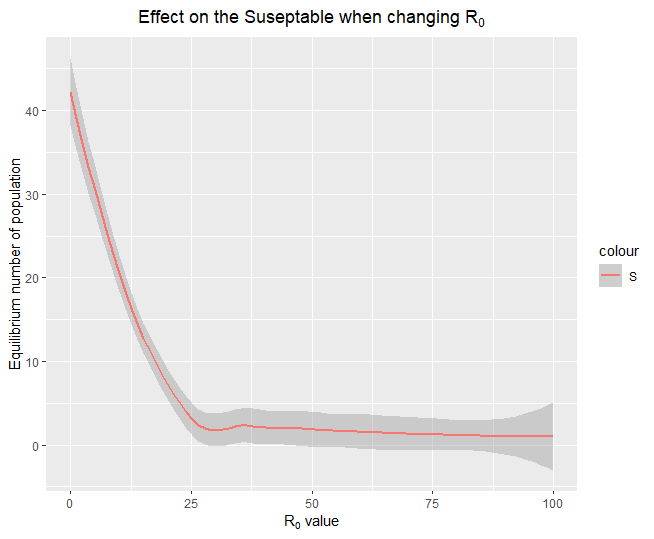
\includegraphics[width=0.45\textwidth]{./figures/MarioPlt/R0Sus.png}
      \end{center}
\caption{The affect of changing $R_0$}
\end{figure*}

\noindent
$R_0$ affects a number of things, mainly the gradient of the first peak, the time between waves and the height of the first peak. This makes sense, because, in a biological sense, the $R_0$ number is the amount of people a single person infects. We decided to set the $R_0$ value to follow what it was modelled as in reality during first wave of the SARS-CoV-2 virus pandemic, which was approximately 1.6 \cite{reprodnumber}. As $R_0$ increases, there are more people infected and less susceptible, so the equilibrium number of susceptible are lower (as shown in Figure 2). \\

\noindent
Other variables influencing our model are $t_O$ and $t_Y$; these increase and decrease the time that a patient has the disease, so this variable is strictly greater than $0$.






We shall also note that the effect on the behaviour of the model doesn't change if we consider $t_O$ or $t_Y$, and so we will consider $t_O$. As you increase $t_O$ the behaviour fits into three different kinds, these are achieved when $0 < t_O < 1$, $1 < t_O < 17$ and $17 \le t_O$, so we will consider three different values of $0.5, \, 5$ and $30$, we will see that the number of people recovering per unit time is decreased, and instead they spread over a longer period. Let us fix $R_0 = 1.6$ and $t_Y = 7.6$.\\


\begin{figure*}[ht!]
\begin{center}
      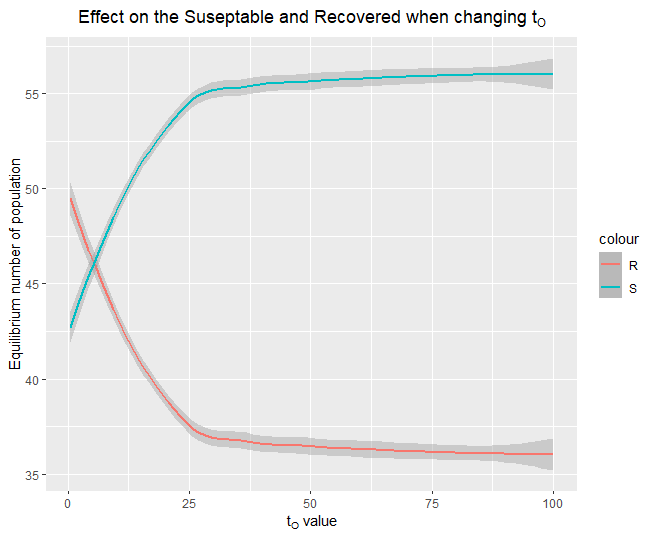
\includegraphics[width=0.45\textwidth]{./figures/MarioPlt/tOSusRec.png}
      \end{center}
\caption{The affect of changing $t_O$}
\end{figure*}

\newpage
\noindent
As expected we see that we have a decrease in the number of individuals recovering per unit time and the peak of recovered is moved forward with the increase in $t_O$. We also see that the peak of infected individuals is broader and is moved forward to a limit point of $t \approx 50$ as $t_O \to \infty$. Thinking in a biological context, these are simply just corollaries of the patient being infected for longer as people would infect a higher number of other people (hence, an increase in area under the infected graph) and there will be a longer time until people recover, hence the oscillatory nature of the recovered curve in the second graph. \\
\noindent
As we know that $\displaystyle{R_0 = \frac{\beta}{\sigma + \delta}}$ and we assume that $R_0$ is the same for each part of the population.\footnote{This is a bit of an oversight, we should really say that we take a matrix $\mathbf{G}$ of all the different $R_0$'s for each mixing of population and then find the spectral radius, i.e. dominant eigenvalue of the matrix. \cite{r0paper}}
 We then set $\sigma \approx \frac{1}{t_O}$ or $\sigma \approx \frac{1}{t_Y}$. Hence we can use the above graphs to show what the effect of changing the $\sigma$s do to the model. Given, we intertwine the two parameters, but that matters little as we set these parameters given data about SARS-CoV-2.\\
 
\noindent
The $d_1$ and $d_2$ parameters define the daily death rate for the infected in each population, so are required to be within 0 and 1. Using data from the literature, we calculated the average daily death rate of the under 80s and of 80s groups in the UK to be, $d_1 = 0.001= 0.5,\text{ and } d_2 = 0.05$, the death rate being much higher for the old population. In our model, due to %due to vaccination distribution changing and% <- FYI this is commented out so won't appear in the document/ yeye, thought it might be good to add after V_ is added
reductions in cross-infections, increasing death rate in one population reduces the death toll in the other. If $d_2 > i_2\text{ (infection rate) }$ then the virus will on average kill it's host before spreading, so will fail to disseminate across the population. Figure 4 considers the death factor $\delta$ for the total population between 0 and 1.

\begin{figure*}[ht!]
\begin{center}
      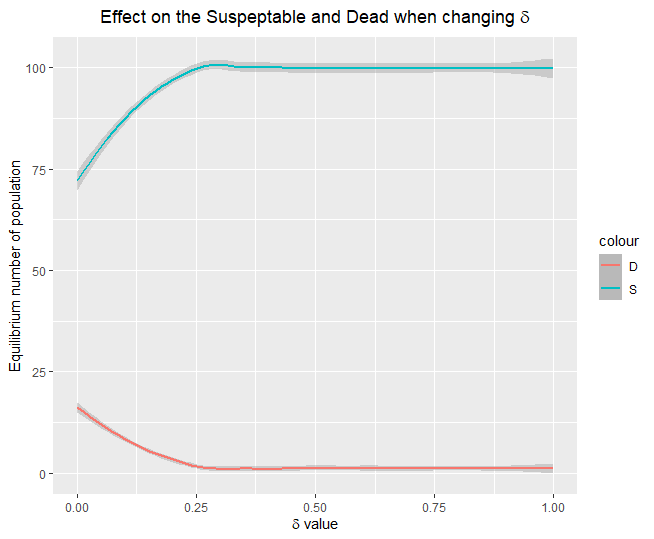
\includegraphics[width=0.45\textwidth]{./figures/MarioPlt/dSusDed.png}
      \end{center}
\caption{The affect of changing $\delta$}
\end{figure*}



\noindent
The death rate is more consistent with a $\delta$ closer to 1
since infections from both infected populations remain high. 
As $\delta$ increases the proportion of deaths fall in the population as the lethality of the disease reduces the rate of infection of the virus, so less individuals are able to be killed by the virus.





\noindent
The final parameters of the SIRD model are the $\iota$ parameters $\iota_1$ and $\iota_2$, the rate at which people lose immunity to the virus. These parameters are defined as,
$$\iota_i = \displaystyle{\frac{1}{\text{days of immunity for $i$}}}$$ 
%Immunity time post-infection with COVID-19 is relatively consistent between age groups and lasts on average for 5 months \cite{ImmuneTimeRecovered}. 
As the parameters relate to 1 over time in days, any values between 0 and 1 may be used.

\newpage
\begin{figure*}[ht!]
\begin{center}
      \includegraphics[width=0.45\textwidth]{./figures/MarioPlt/iInfded.png}
      \end{center}
\caption{The affect of changing $\iota_0$}
\end{figure*}

\noindent
As $\iota$ decreases, the severity of the first wave is reduced and so the time between the first and second waves increases. As a result, reduction in $\iota$ reduces the rate of death during the epidemic (total deaths however in this closed SIRD model will always eventually reach 100\%).


% blah blah blah, this one just moves the peak of infections down and right and the recovered up and right. This is what we expect blah blah blah


% incubation periods




\newpage
\subsection{Optimisation}
Once we had a model in place and had mapped all of the parameters, we could focus on what the optimal vaccination strategy was. As we had two populations we could define the percentage of population that is vaccinated by $p$, and this we named the vaccination factor. We defined the amount of the population vaccinated on a certain day as,
\begin{align*}
    V_Y &= p V_{max} \\
    V_O &= (1 - p)V_{max}
\end{align*}
and since we fixed the total number of vaccinations given out each day, $0 \le p \le 1$. Here we had the beginning of an optimisation problem, as we studied in Part I of the course. We had a choice of what to optimise: either we minimised the deaths, minimised the cases or a mixture of both. We also could weight the cases and death from a population as we have, $S_1, S_2, D_1$ and $D_2$.\\

\begin{minipage}{0.45\textwidth}
\begin{algorithm}[H]
\SetAlgoLined
\KwResult{Optimal Vaccination factor to 4.s.f}
 let $a = 0$, $b = 1$, $i = 0$\;
 \While{$i < 4$}{
  potSol = linspace($a$, $b$, $11$) \;
  \For{$j$ in potSol}{
  calculate the $\nu$ factors for each population\;
  solve the SVIRD model with $\nu_1$ and $\nu_2$\;
  oF = compute the objective function\;
  sols.append(oF)\;
  }
  $a = \text{max(sols)} - \frac{1}{10^i}$\;
  $b = \text{max(sols)} + \frac{1}{10^i}$\;
 }
 print(max(sols))
 \caption{Optimisation Algorithm}
 \captionof{figure}{Optimisation Algorithm}
\end{algorithm}
\end{minipage}
\hspace{\fill}
\begin{minipage}{0.45\textwidth}
  We then had to find an optimal $p$, and so we chose a mesh of $\{0, 0.1, \dots, 1\}$ and run simulations for each of these. Then we chose the one with the minimal objective function. Then after we found an optimal for the course mesh, the programme worked it's way down to finer and finer meshes. As you can see in the psudocode to the left, we chose to just go to 4s.f. as this provided a suitable accuracy, and going much further would increase computation without offering considerably more information. \\
  
  This method is called a bisection method and is a very naive algorithm, however our problem is rather simple. We just want to take some inputs and find which output is optimal. 
\end{minipage}

\newpage
\section{Results and Discussion}
\subsection{Vaccination Scenarios 1 - Once vaccinated, always immune}

\noindent
This is the simplest scenario. The model assumes the vaccination gives ever-lasting immunity from the virus, meaning once an individual moves into the vaccinated group of the model, they do not re-enter the susceptible group. Although unlikely in reality, this scenario informs us of the initial patterns of the infection rate and death rate after the vaccination, when a level of immunity is guaranteed. The vaccination scheme is modelled to start at time unit (day) 200, reflecting the real-life delay for vaccinations to be made and distributed, and for the optimised ratio to give the older population 90\% of the vaccinations and the younger population 10\%. Figure 7 shows that after the vaccinations begin, the infection and death rates drop dramatically in both populations, as expected. However it is worth highlighting that the proportion of deaths was considerably bigger in the older population (approximately 33.2\% died in the older population and 10.1\% in the young population). Hence a larger proportion of the vaccinations should be given to the older population, since our model suggests older people (those over 80 years) are more likely to die from the virus than the younger people (below the age of 80 years). This aligns with current literature and research on the SARS-CoV-2 virus \cite{mightdieyouoldie}.
\noindent
These patterns therefore support our optimisation result to give 90\% of the vaccinations to the older population first of all.

\begin{figure*}[ht!]
   \subfloat{%
      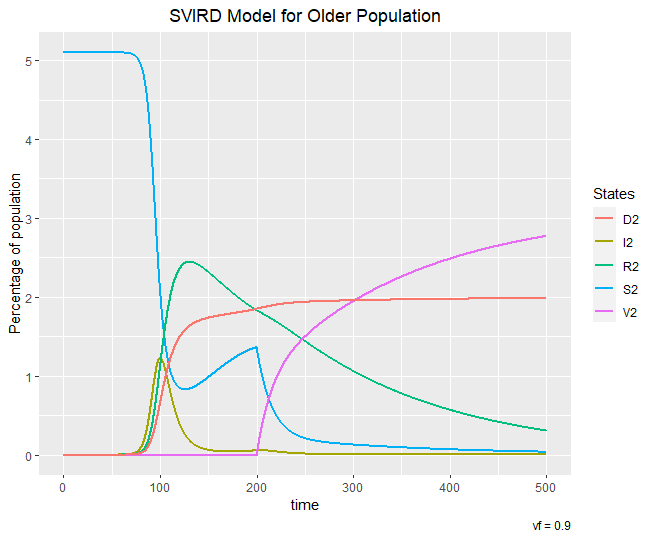
\includegraphics[width=0.45\textwidth]{./figures/scenarios/scen1/OldScen1.png}}
\hspace{\fill}
   \subfloat{%
      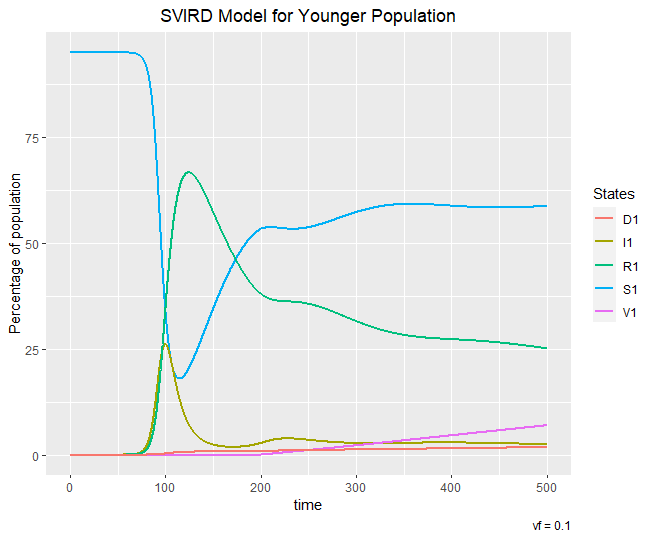
\includegraphics[width=0.45\textwidth]{./figures/scenarios/scen1/YoungScen1.png}}
\caption{Scenario 1 for both populations}
\end{figure*}






\subsection{Vaccination Scenario 2 - Living with SARS-CoV-2}

Our second Scenario also considered the SARS-CoV-2 virus, and followed a simulation of the UK outbreak. This test involved a vaccine that wasn't 100\% effective. Our parameters for this model aimed to recreate the characteristics of the disease. %do we include parameters used & evidence for that?
\noindent
In this optimum simulation, a larger second wave was avoided in the over 80s population through the vaccination effort being focused on them $9:1$, reducing the second peak of susceptible individuals. This response was likely favoured due to the age-related lethality of the virus, repeating the top-down vaccine response followed in the UK. 
A result of the addition of an imperfect vaccine revealed a 'living with COVID-19' scenario, where vaccinations can never be distributed to the whole population due to logistical limitations. In this scenario, deaths continue on an upward curve and vaccinations are maintained in an optimum ratio in the populations to reduce deaths. The deaths were a lot higher in this scenario with approximately 47.1\% of the over 80s in the population dying and 2.1\% of the under 80s dying in 500 days.

% Deaths following upward curve
% Lots more deaths
% Equilibrium reached a lot later in the curve
% Implies critical mass of vaccination, question here to what level need to be vaccinated in order to reach a stable state as Old people reach a SS while younger population is far off a SS. DONT KNOW HOW TO WORDdddd

\begin{figure*}[ht!]
   \subfloat{%
      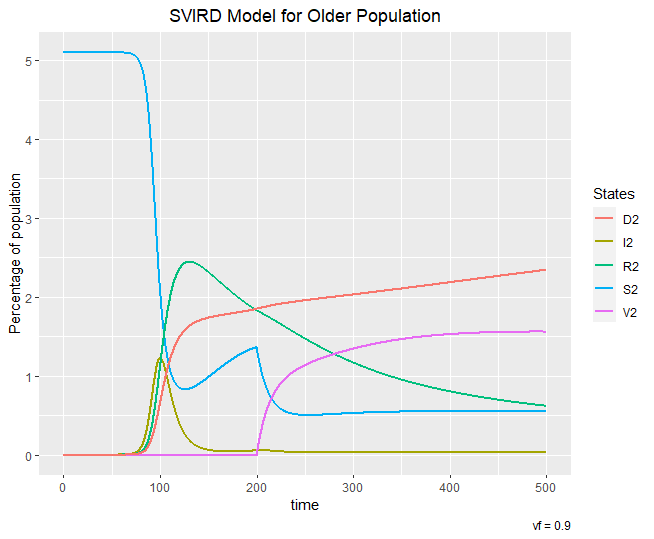
\includegraphics[width=0.45\textwidth]{./figures/scenarios/scen2/OldScen2.png}}
\hspace{\fill}
   \subfloat{%

      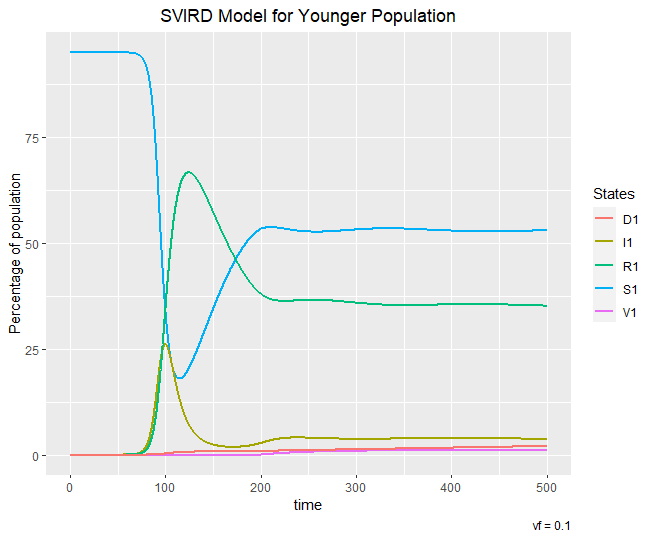
\includegraphics[width=0.4\textwidth]{./figures/scenarios/scen2/YoungScen2.png}}
\caption{Scenario 2 for both populations}
\end{figure*}


\newpage
\subsection{Vaccination Scenario 3 - 25\% being asymptomatic}
A very recent study has shown that people with the vaccine are only asymptomatic 25\% of the time\cite{cit1}. This is something we can add to our model! Vaccinated people will have the mentality that they are not carrying the virus and immune to it, hence the mixing factors for them will be higher than for the non-vaccinated people. We can hence adapt our $\underline\beta$,
$$ \underline{\beta} = \begin{pmatrix} 
  \frac{R_0}{t_Y} & \frac{1}{2}\left ( \frac{R_0}{t_Y} + \frac{R_0}{t_O} \right ) & \frac{R_0}{4t_Y}\gamma_C\\
  \frac{1}{2}\left ( \frac{R_0}{t_Y} + \frac{R_0}{t_O} \right ) & \frac{R_0}{t_O} & \frac{R_0}{4t_O}\gamma_C
\end{pmatrix}
$$
these new factors implement that evidence that 25\% of people vaccinated (with PfizerBionTech vaccine, which we will assume for brevity that the vaccine being administered), can still be asymptomatic or carriers of SARS-CoV-2. Hence, we now have a slightly altered model, with new factors. $v_j$ is the rate of people doing from $V_j$ to $S_j$.

    \begin{figure}[!ht]
      \centering
      \scalebox{.9}{\begin{tikzpicture}[node distance=2.5cm, auto,
      >=Latex,
      every node/.append style={align=center},
      int/.style={draw, minimum size=1cm}]

     \node [int] (S)             {$S_j$};
     \node [int, above=of S] (V) {$V_j$};
     \node [int, right=of S] (I) {$I_j$};
     \node [int, above=of I] (D) {$D_j$};
     \node [int, right=of I] (R) {$R_j$};
     \coordinate[right=of I] (out);
     \path[->] (S) edge node {$\beta_{j1} + \beta_{j2} + \beta_{V}$} (I)
               (R) edge[out=-120, in=-60] node {$\iota_j$} (S)
               (I) edge node {$\delta_j$} (D)
               (S) edge node {$\nu_j$} (V)
               (V) edge node {$v_{j}$} (S)
               (I) edge node {$\sigma_j$} (R);
    \path[dashed] (V) edge node {} (I);
  \end{tikzpicture}}
      \caption{A more accurate SVIRD model for a population $j$}
      \label{fig:SVIRDrealLife}
    \end{figure}

\noindent
From this we can then get the following simulations, which are very interesting. As before we had simulations where the vaccinations were preferred for the older population, in these simulations the younger population are preferred. 

\begin{figure*}[ht!]
   \subfloat{%
      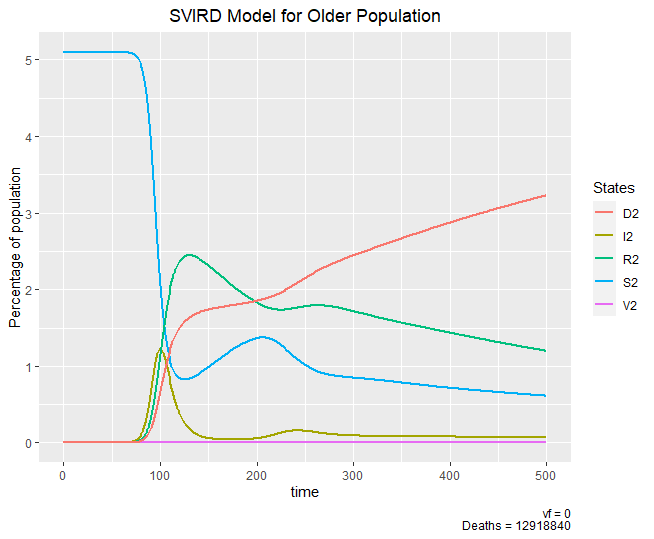
\includegraphics[width=0.45\textwidth]{./figures/scenarios/scen3/OldScen3.png}}
\hspace{\fill}
   \subfloat{%

      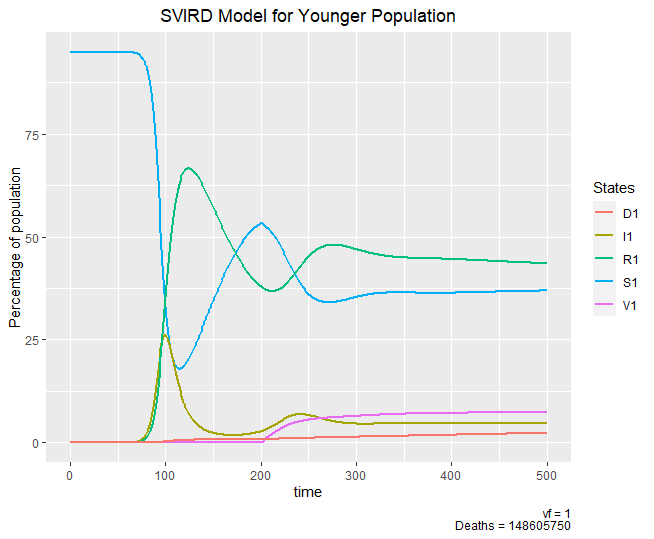
\includegraphics[width=0.45\textwidth]{./figures/scenarios/scen3/YoungScen3.png}}
\caption{Scenario 3 for both populations}
\end{figure*}

\noindent
This presents an extreme contrast to the previous scenarios, here we are trying to minimise death of the population, through vaccinating the biggest spreaders, the younger population. Here we had to introduce a new mixing factor which we are calling $\beta_{jV}$ which is equal to the mixing factors of people in the same population multiplied by some cofidence factor $\gamma_C$ ($1 < \gamma_C < 2$). In this range the results are the same, however past $2 < \gamma_C$ we get a larger second peak and as $\gamma_C \to \infty$ which would be an example of a lockdown, then the correct vaccination strategy converges back to the previous situation.\\



\subsection{Limitations}
\noindent
The largest limitation to our model is its assumption that all sub-age groups below 80 years in the younger population respond similarly to the virus, however in practice this is not true. People in the age group 40-80 years experienced more intense symptoms to the virus than people aged under 40. Although, not considered here, it is possible for a further study to develop the model set out in this study, by dividing the population into more sub-populations. However, this introduces more parameters and increases the complexity of each conclusion, so considering the time frame this project was under, the model focuses on the most extreme difference in symptom intensity- that between populations under and over 80 years old.\\

\noindent
Our model assumes that the usual rate of mixing within the population continues, and so the transmission rate remains constant. This means our model doesn't account for lock downs or people following government rules (6-people mixing), and assumes no change of behaviour if a person gets infected i.e. they do not self-isolate. In reality, these factors have been shown to limit the transmission rate greatly and decrease the rate of which the virus is spreading. This makes our model less representative, but again, in light of the time constraint this project was under, it would not be feasible to heighten the complexity to this extent.\\

\noindent
Another limitation of our model is that it gives full immunity to the individual after one vaccination. This doesn't represent what actually happens in reality since most SARS-CoV-2 vaccinations (such as the Oxford AstraZeneca vaccine), require two jabs 12 weeks apart, and give 82.4\% immunity \cite{astravaccine}. 

This limits the reliability of the model, since it would, in reality, take longer for the vaccine to give immunity and at a lower certainty of immunity than the model predicts. To include this in our model, we could develop the vaccination group into stages, and consider only transferring 82.4\% of people vaccinated to the vaccinated group from the susceptible group. \\

\noindent
A limitation of the model is that it only models the first strain of the SARS-CoV-2 virus. Although this was sufficient to model the initial characteristics of the virus, a future model may incorporate the different strains of the virus to achieve a more representative model. 

\section{Conclusion}
%1 outline
This work set out to create a SIRD model that could be used and adapted to explore the managing of a disease outbreak using a vaccine. The model created incorporates another level of complexity by dividing the target population into two age groups, allowing different characteristics between age groups of the modelled disease. This model would then be applied to a variety of scenarios to judge optimal vaccine responses in these events, even applying the latest research to the model on the probability of vaccinated asymptomatic individuals, displaying the adaptability of the model we created. \\

\noindent
%2 Summary of results
The SVIRD model created, successfully displays disease scenarios with recognisable features such as first and second waves, death rate stagnation due to resistance and the results of a nationwide vaccine response. Our results show that the model is applicable in forecasting disease spread and optimising vaccine response strategies between two connected populations. Due to limitations in the simplicity of the model it cannot be used to predict accurately the rate of infection and death from diseases such as COVID-19. However, it is usable in its application of discovering the dynamics of a pandemic with regards to the variables within the model and any added in future simulations. 
For example in Scenario 2, with the implementation of incomplete immunity from the vaccine in the model, the disease is not eradicated from the population. This shows a similar outcome to how known diseases, such as measles, have to be managed for the foreseeable future in a population and that vaccinations of susceptible \& vulnerable individuals must be prioritised. In this scenario, under parameters defined by COVID-19 literature, individuals over 80 were heavily prioritised to reduce deaths at $9:1$. In Scenario 3, the addition of asymptomatic vaccinated carriers for the disease being super-spreaders for the virus caused the optimal vaccination effort to focus on under 80s, with 100\% of vaccines going to that group to reduce overall deaths. The nature of the outbreak also displays how the virus may not be able to be eradicated due to how the virus is spread by asymptomatic carriers unlike small pox, a disease that has been eradicated in many places \cite{smallpx}. \\

\noindent
This work has provided evidence supporting the claim that, to minimise the number of deaths in the SARS-CoV-2 virus outbreak, the majority of the initial vaccinations should be assigned to the older population group (of age 80+ years). Therefore, when deciding whether prevention or protection techniques should be adopted for the SARS-CoV-2 virus outbreak in the UK, we should prioritise protection techniques, i.e. vaccinating the older populations first (or in a majority).



\newpage
\section{Bibliography}
\printbibliography


\end{document}
